\documentclass{article}
\usepackage[utf8]{inputenc}
\setlength\parindent{0pt}
\usepackage{hyperref}
\usepackage{graphicx}
\usepackage{float}
\usepackage{amssymb}
\usepackage{amsmath}


\begin{document}

\begin{figure}[H]
    \centering
    
\includegraphics[width=0.8\textwidth]{images/TUe-new-logo.png}
\end{figure}

\vspace{1.2cm}

\begin{center}
\huge{A very brief history of\\ \textbf{convolutional neural networks}}\\

\vspace{0.5cm}

\Large{Bram Grooten (0885158)}\\

\vspace{0.2cm}

\Large{June 2020}\\

\vspace{1.4cm}

\begin{figure}[H]
    \centering
    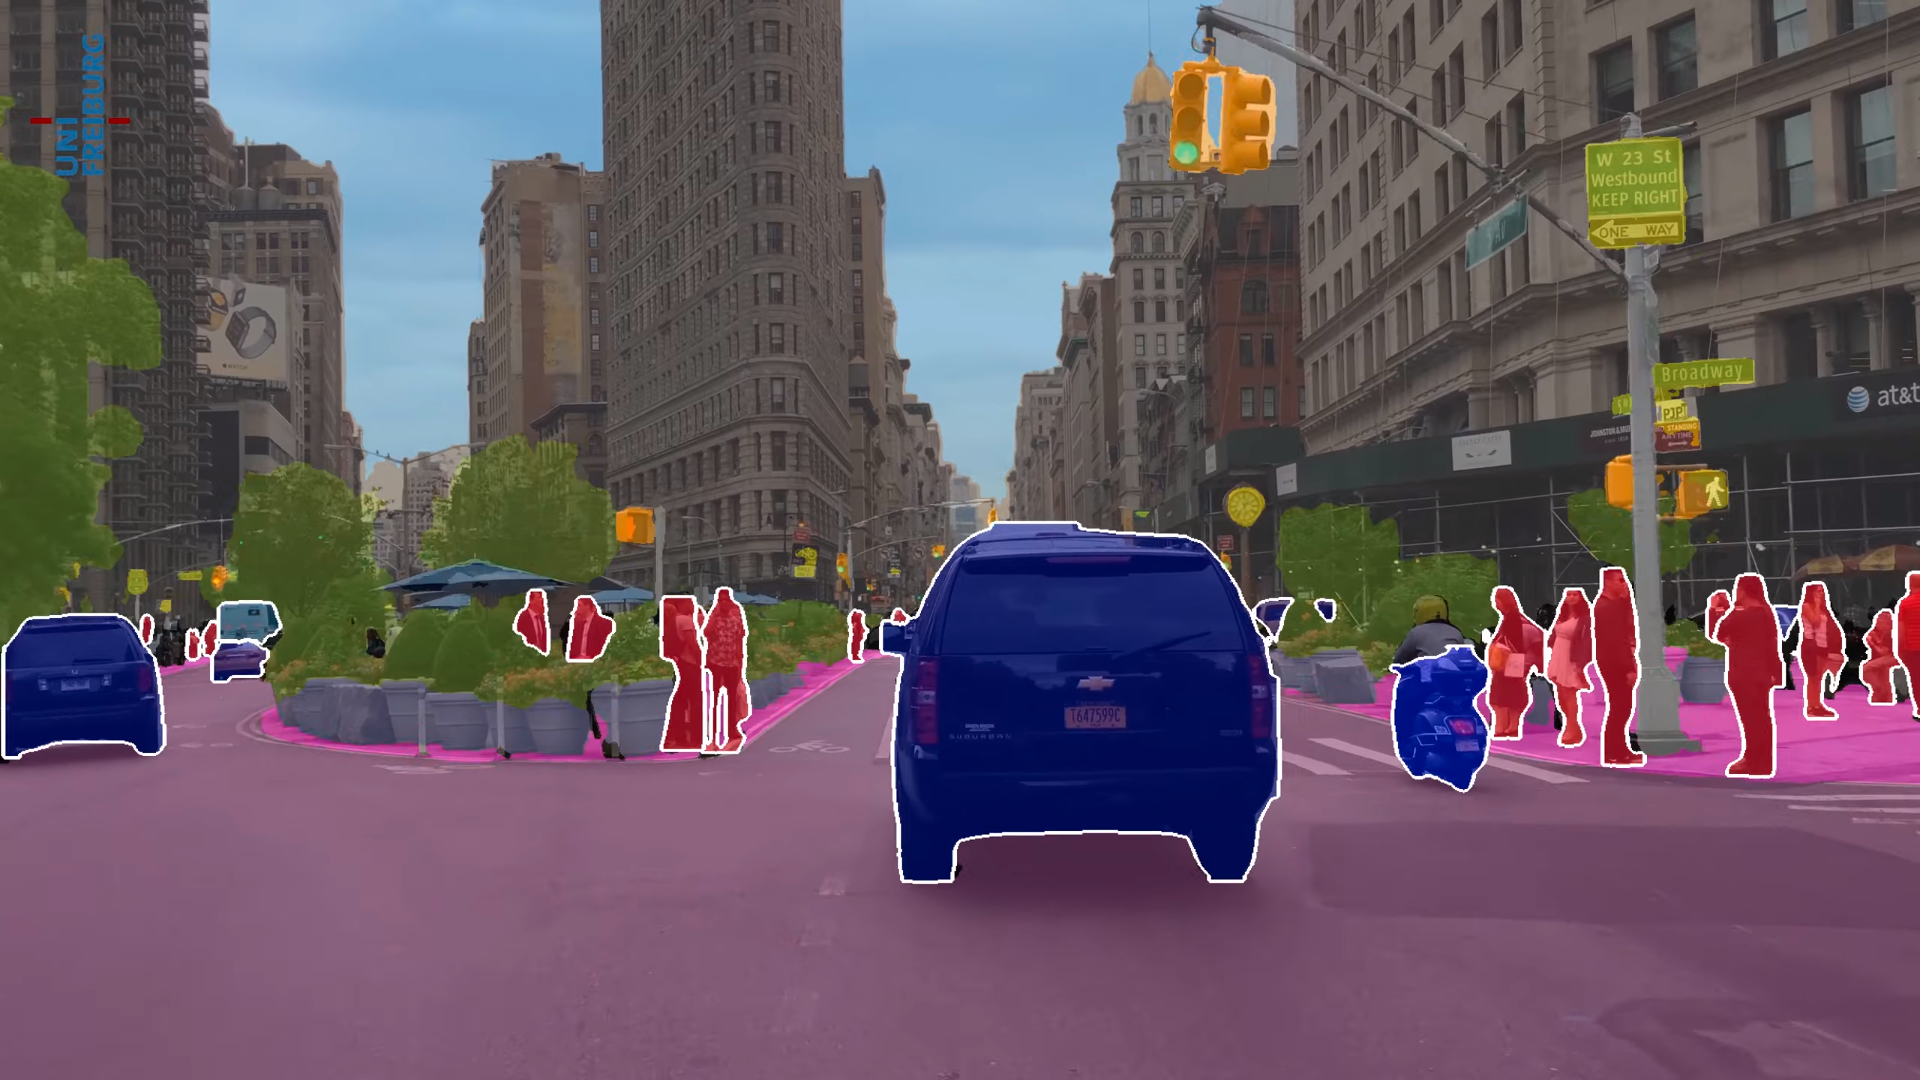
\includegraphics[width=\textwidth]{images/effPS-still23m12s.png}
\end{figure}

\vspace{1.4cm}

Mathematics and practice in historical perspective (2WH60)
\end{center}


\newpage
Cover image \cite{effps}: object recognition for self-driving cars is an application of deep learning where convolutional neural networks are used.


\vspace{1cm}

\tableofcontents

\vspace{1cm}


\section{Introduction}

In deep learning, which is a subfield of artificial intelligence \cite[Ch. 1]{dl-book}, % page 9
different kinds of artificial neural networks are used for numerous applications. This paper will look at the history of a specific type of network: the convolutional neural network (CNN). The main goal is to discover the mathematical foundations of CNNs and describe the corresponding historical development. Other questions that we will explore throughout the paper are: What is a CNN? Who invented it? What are the applications? The answers will always be given with an overview on the historical perspective.



\section{What is a convolutional neural network?}

To answer the question of what a convolutional neural network is, we first need to understand the basics of a neural network. The term already contains some information: it is a network of neurons. These neurons can be either biological: in the brain of an animal, or artificial: as part of a computer program.\\

\subsection{Artificial neurons}

The artificial neuron behaves similar to the biological neuron. They both take a number of inputs, which combined with the settings of the neuron, give a specific output. Mathematically speaking, an artifical neuron is just a function. It takes a number of input values and computes the corresponding output based on the current setting of the neuron. The setting of a neuron can change over time. When a neural network is \textit{learning}, it is making adjustments in the settings of its neurons.\\

The first mathematical model of an artificial neuron was proposed by McCulloch and Pitts in 1943 \cite{first, mcc}. The model, shown in \autoref{fig:mp}, was similar to a logic gate and is now often called the threshold logic unit (TLU). In 1958 Rosenblatt improved the TLU into his \textit{perceptron} \cite{percep}, which works as follows. A number of input values $x_1, \ldots, x_n \in \mathbb{R}$ reach the neuron. The neuron computes a value based on the setting of its weights $w_1, \ldots, w_n \in \mathbb{R}$:
\begin{equation*}
    g(x_1, \ldots, x_n) = \sum_{i=1}^n w_i x_i = v.
\end{equation*}
This value $v$ gets compared to a threshold $\theta$ by a function $f$:
\begin{equation}
    f(v) = 
    \begin{cases}
        1 & \textbf{if } v > \theta \\
        0 & \textbf{if } v \leq \theta
    \end{cases}
\end{equation}
which becomes the output value $y$ of the neuron. This second function is often called the activation function of a neuron. It determines whether the artificial neuron ``fires". Nowadays there are many possible activation functions, some allowing $y$ to take on any value in $\mathbb{R}$.\\

\begin{figure}
    \centering
    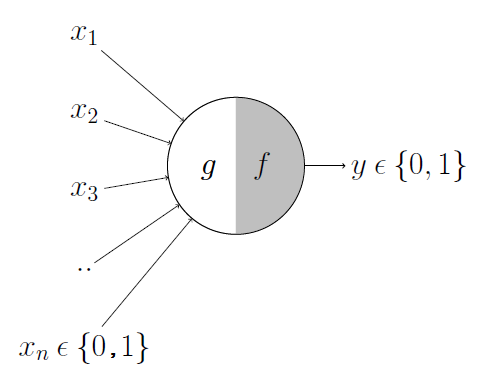
\includegraphics[width=0.8\textwidth]{images/mp.png}
    \caption{The threshold logic unit by McCulloch and Pitts. Source: \cite{med}}
    \label{fig:mp}
\end{figure}

A neural network arises when many of such artifical neurons are connected together. If the output of each neuron in one layer serves as the input to every neuron in the next layer (forming a complete bipartite graph) then these layers are called fully connected. When all the layers have this property, it is a fully connected neural network, such as the example in \autoref{fig:full}.\\

\begin{figure}
    \centering
    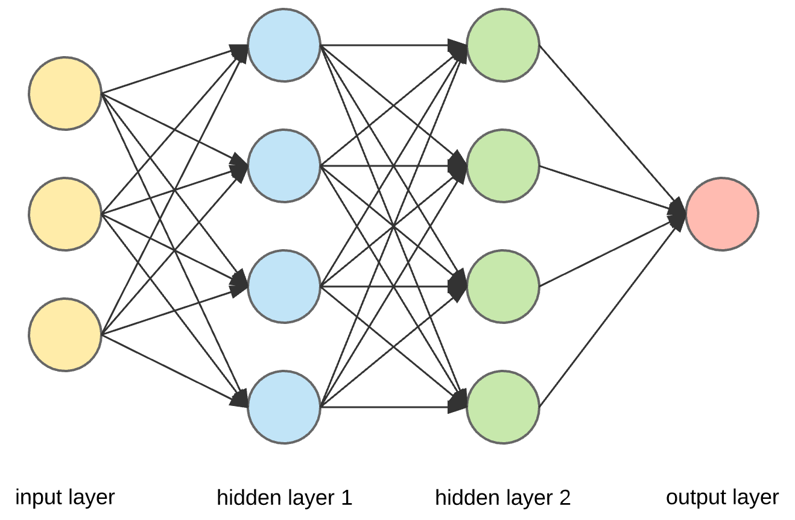
\includegraphics[width=0.8\textwidth]{images/fullyNet.png}
    \caption{An example of a fully connected neural network. Source: \cite{fullpic}}
    \label{fig:full}
\end{figure}

\subsection{Convolutional}

Convolutional neural networks differ from regular neural networks in a couple of ways. First of all, they are much sparser in their connectivity, which means that a neuron is not influenced by all the neurons in the previous layer. However, particular neuron can still depend on all the values of a deeper layer indirectly, as shown in \autoref{fig:indir}.\\

\begin{figure}
    \centering
    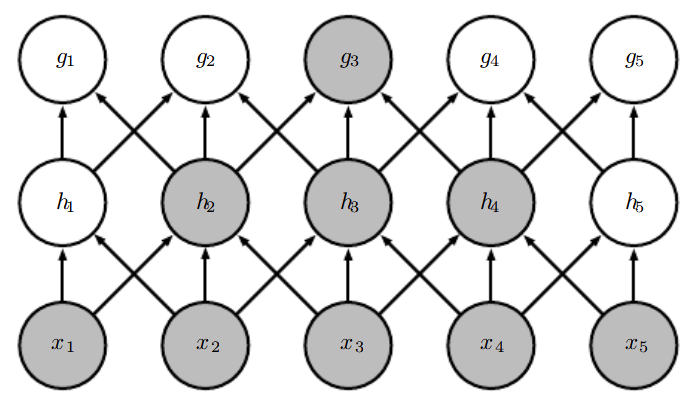
\includegraphics[width=0.8\textwidth]{images/indir.png}
    \caption{Neuron $g_3$ is indirectly influenced by all output values of a deeper layer. Source: \cite{dl-book}}
    \label{fig:indir}
\end{figure}

Another difference, from which CNNs derive their name, is the fact that CNNs use the convolution operation instead of regular matrix multiplication. More on this in \autoref{sec:math}. A neural network is called convolutional, if at least one of its layers uses the convolution operation \cite[Ch. 9]{dl-book}. There can still be some fully connected layers in a CNN.\\

%% eerst nog een stukje over hoezo regular matrix multiplication









\section{Who invented CNNs and why?}

It is a little difficult to answer this question directly and clearly. There are of course multiple people who have contributed to the advancements that led to the convolutional neural networks of today. In this section we will look at a couple of important people who made the biggest contributions, and try to discover what motivated them towards the inventions.\\

\subsection{Kunihiko Fukushima}

The neural network that many consider as the root of convolutional networks was the neocognitron. Some say this was the first CNN \cite{sch, fuzzy}, while others call it the inspiration that led to CNNs \cite{dl-lecun, history}. Anyhow, the neocognitron was invented in 1979 by Kunihiko Fukushima. It was first described in a Japanese paper \cite{jap} and one year later he published an English version on the same topic \cite{neocog}. Let us have a look at the man himself.\\

Fukushima, shown in \autoref{fig:fuku}, was born in 1936 \cite{about-fuku} on the island of Taiwan, which was under Japanese rule at the time. His family moved to Japan after the second world war. He became interested in electronics when an uncle gave him a disassembled electric motor to play around with. Little Kunihiko built a radio and even an electric train. This might have motivated him to study Electronics for his bachelor at Kyoto University, which he finished in 1958. Later on in 1966 he would also achieve his PhD there.\\

\begin{figure}
    \centering
    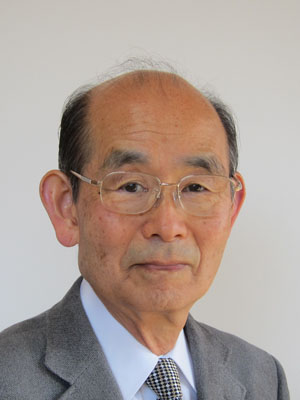
\includegraphics{images/Fukushima.jpg}
    \caption{Kunihiko Fukushima, the inventor of the neocognitron. Source: \cite{fuzzy}}
    \label{fig:fuku}
\end{figure}

During his PhD, Fukushima joined a research group on visual and auditory information processing at Japan's national broadcasting company NHK. He worked together with neurophysiologists to investigate the biological brain, which is the final destination of broadcasted signals. He was especially interested in modelling the higher brain functions, like the visual system, and applying that to an artificial neural network \cite{fuzzy}. He has received multiple awards for the neocognitron he came up with, and his further work on neural networks.  Extensions of his neocognitron are still being developed, and Fukushima himself is also still publishing. Just last year (2019) at the age of 83 he wrote about reducing the computational costs of a deep neural network \cite{83}.\\

Working together with neurophysiologists contributed to Fukushima's invention of the Neocognitron. In his paper \cite{neocog} he specifically mentions the inspiration coming from the discoveries of Hubel and Wiesel. These two men uncovered the hierarchical, layered strucuture of the visual cortex while studying the brains of cats in the early 1960's \cite{hubel, wiesel}.


\subsection{Yann LeCun}



\subsection{Other major advancements}


Weng (1993) later replaced Spatial Averaging by "Max-Pooling" (MP), which is widely used today \cite{sch}.
% eigen woorden nog

Ranzato et al. (2007) first applied BP to Max-Pooling CNNs (MPCNNs); \cite{sch}



\section{What are the mathematical foundations of a CNN?}
\label{sec:math}


\section{What are the practical applications of CNNs?}


















\begin{thebibliography}{}



\bibitem{effps} R. Mohan and A. Valada. (2020). \textit{EfficientPS: Efficient Panoptic Segmentation}. \url{http://panoptic.cs.uni-freiburg.de/}

\bibitem{dl-book} I. Goodfellow, Y. Bengio and A. Courville. (2016). \textit{Deep Learning}. MIT Press. \url{http://www.deeplearningbook.org/}

%% soms hoofdstuk 1, soms hfst 9: fix dit in de tekst 


\bibitem{first} \url{http://historyofinformation.com/detail.php?entryid=782}

\bibitem{mcc} McCulloch, W. S., \& Pitts, W. (1943). A logical calculus of the ideas immanent in nervous activity. The bulletin of mathematical biophysics, 5(4), 115-133.

\bibitem{percep} Rosenblatt, F. (1958). \textit{The perceptron: A probabilistic model for information storage and organization in the brain}. Psychological Review, 65(6), 386–408. https://doi.org/10.1037/h0042519

\bibitem{med} https://towardsdatascience.com/mcculloch-pitts-model-5fdf65ac5dd1

\bibitem{fullpic} \url{https://www.linkedin.com/pulse/deep-learning-nutshell-part-1-ankit-agarwal/}

\bibitem{dl-lecun} LeCun, Y., Bengio, Y. & Hinton, G. \textit{Deep learning}. Nature 521, 436–444 (2015). \url{https://doi.org/10.1038/nature14539}

\bibitem{jap} K. Fukushlma, Neural network model for a mechamsm
of pattern recognmon unaffected by shift m
posltlon--neocogmtron--, Trans Inst electromcs commun
Enors Japan 62-A, 658-665 (1979) (In Japanese)

\bibitem{neocog} K. Fukushima, \textit{Neocognitron a self-organizing neural
network model for a mechanism of pattern recognition
unaffected by shift in position}, Biological Cybernetics 36,
193-202 (1980)

\bibitem{sch} Schmidhuber, Jürgen (2015). "Deep Learning". Scholarpedia. \url{http://www.scholarpedia.org/article/Deep_Learning}

\bibitem{about-fuku} "Kunihiko Fukushima". The Franklin Institute. \url{https://www.fi.edu/laureates/kunihiko-fukushima}

\bibitem{fuzzy} \url{http://personalpage.flsi.or.jp/fukushima/index-e.html}

\bibitem{history} \url{https://www.import.io/post/history-of-deep-learning/}

\bibitem{83} Fukushima, K. (2019). Efficient IntVec: High recognition rate with reduced computational cost. Neural Networks, 119, 323-331.

\bibitem{hubel} Hubel, D.H., Wiesel, T.N. \textit{Receptive fields, binocular interaction
and functional architecture in cat's visual cortex}. J. Physiol.
(London) 160, 106-154 (1962)

\bibitem{wiesel} Hubel, D.H., Wiesel, T.N. \textit{Receptive fields and functional architecture in two nonstriate visual area (18 and 19) of the cat}. J.
Neurophysiol. 28, 229-289 (1965)

\bibitem{wolf} \url{https://mathworld.wolfram.com/Convolution.html}

\bibitem{tor} \url{https://www.slideshare.net/Alexdfar/origin-adn-history-of-convolution}

\bibitem{stanf} \url{http://ufldl.stanford.edu/tutorial/supervised/FeatureExtractionUsingConvolution/}







\bibitem{fake} \url{https://thispersondoesnotexist.com/}















\end{thebibliography}

\end{document}
